\documentclass{ws-jcsc}
\usepackage{amsmath,amssymb}
\usepackage{graphicx}
\usepackage{tikz}
\usetikzlibrary{positioning,arrows.meta}
\usepackage{booktabs}
\usepackage{multirow}
\usepackage{url,overcite}
\usepackage{xcolor}
\usepackage[verbose]{hyperref}
\hypersetup{colorlinks=false,allbordercolors=blue,pdfborderstyle={/S/U/W 1}}
\urlstyle{rm}

\begin{document}

\markboth{A. I. Shaposhnikova and S. Tripathi}{Wearable BAC Estimation and Ignition Prevention}

\title{AI-Based Wearable BAC Estimation and\\
Ignition Prevention for Vehicle Safety}

\author{Anastasiia Igorevna Shaposhnikova}
\address{Department of Information Technologies and Engineering,\\
Amity University in Tashkent, Tashkent, Uzbekistan}

\author{Sudhanshu Tripathi}
\address{Department of Information Technologies and Engineering,\\
Amity University in Tashkent, Tashkent, Uzbekistan}

\maketitle

\begin{history}
\received{(Day Month Year)}
\revised{(Day Month Year)}
\accepted{(Day Month Year)}
\published{(Day Month Year)}
\end{history}

\begin{abstract}
This paper presents a software architecture and algorithmic stack for
wearable blood alcohol concentration (BAC) estimation and fail-safe
vehicle ignition control. The system fuses PPG, EDA and temperature
signals on a Wear OS smartwatch, performs on-device inference with a
BiLSTM-attention model, and transmits a 20-byte BAC status packet to an
Arduino-based vehicle controller via BLE. A safety-aware loss function
penalizes false negatives, and a climate-adaptive calibration corrects
for ambient temperature and humidity. Prototype evaluation on synthetic
physiological sequences and a hardware-in-the-loop simulator reports
MAE 0.0082 g/dL, a 0.7\% false negative rate, 580 ms end-to-end latency,
and a 22 KB TensorFlow Lite model. The vehicle-side finite state machine
blocks ignition by default and enforces timeouts and watch-wear checks.
Key limitations include reliance on simulated data and partial
cryptographic enforcement, which define required steps toward clinical
validation and regulatory certification.
\end{abstract}

\keywords{blood alcohol concentration; wearable sensing; sensor fusion;
embedded machine learning; vehicle safety; Bluetooth Low Energy}

\section{Introduction}
Driving under the influence remains a leading contributor to traffic
fatalities, and current enforcement methods are intermittent and easy to
circumvent. Wearable sensing offers continuous monitoring but requires
robust software to estimate BAC from noisy biosignals and to enforce
safety decisions in real time. This paper focuses on the software
methods needed to fuse multimodal wearable data, infer BAC on-device,
and reliably communicate a safety decision to an ignition controller.

The main contributions are:
\begin{itemize}
\item A safety-aware ML pipeline with BiLSTM-attention and an asymmetric
loss to reduce false negatives.
\item A climate-adaptive calibration model for ambient temperature and
humidity effects.
\item A fail-safe BLE protocol and ignition-control state machine that
blocks by default and tolerates communication loss.
\item Prototype evaluation on synthetic data and embedded hardware with
latency and resource measurements.
\end{itemize}

\section{Related Work}
Breath-based ignition interlocks remain the dominant commercial
approach, but require active user participation and are vulnerable to
workarounds. Patented systems describe breathalyzer-triggered ignition
lockout mechanisms\cite{uspat5736965,uspat7113834} and GSM-connected
monitoring\cite{inpat286703}. Transdermal monitoring has matured as a
continuous alternative, with known signal processing demands and
limitations\cite{fairbairn2021}. Recent smartwatch work demonstrates the
feasibility of estimating alcohol exposure from wearable signals\cite{verges2024}.
Embedded breath measurement systems provide additional context for
hardware constraints\cite{lombardo2020}. Vehicle and driver monitoring
research highlights security and tamper resistance requirements\cite{sensors2024,sensors2023}.
Longitudinal EMA frameworks extend monitoring into behavioral studies
and intervention pipelines\cite{alcowatch2025}. These studies motivate a
software-first approach that integrates ML estimation, secure transport,
and fail-safe vehicle control.

\section{System Overview and Requirements}
The system is split across a Wear OS smartwatch and an Arduino Nano 33
BLE controller. The smartwatch acquires PPG, estimated EDA and
temperature signals, performs inference, and broadcasts BAC status. The
vehicle module receives and validates packets, then controls ignition
via a relay. Safety requirements include (i) ignition must be blocked by
default, (ii) BAC over the legal threshold must block ignition, (iii)
watch removal must block ignition, and (iv) loss of fresh BAC data must
block ignition within 60 s.

\begin{figure}[t]
\centering
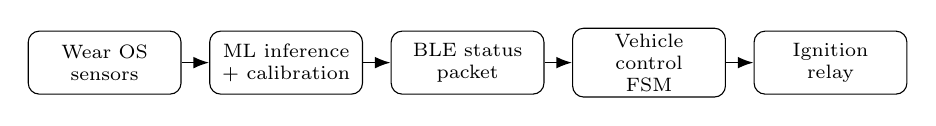
\begin{tikzpicture}[node distance=0.35cm, >=Latex, font=\scriptsize]
\tikzstyle{block} = [draw, rounded corners, align=center, text width=1.8cm, minimum height=0.8cm, inner sep=2pt]
\tikzstyle{link} = [->, line width=0.6pt]

\node[block] (watch) {Wear OS\\sensors};
\node[block, right=of watch] (ml) {ML inference\\+ calibration};
\node[block, right=of ml] (ble) {BLE status\\packet};
\node[block, right=of ble] (vehicle) {Vehicle control\\FSM};
\node[block, right=of vehicle] (relay) {Ignition\\relay};

\draw[link] (watch) -- (ml);
\draw[link] (ml) -- (ble);
\draw[link] (ble) -- (vehicle);
\draw[link] (vehicle) -- (relay);
\end{tikzpicture}

\caption{System overview: wearable sensing, on-device inference, BLE
transport and vehicle-side ignition control.}
\label{fig:system}
\end{figure}

\begin{figure}[t]
\centering
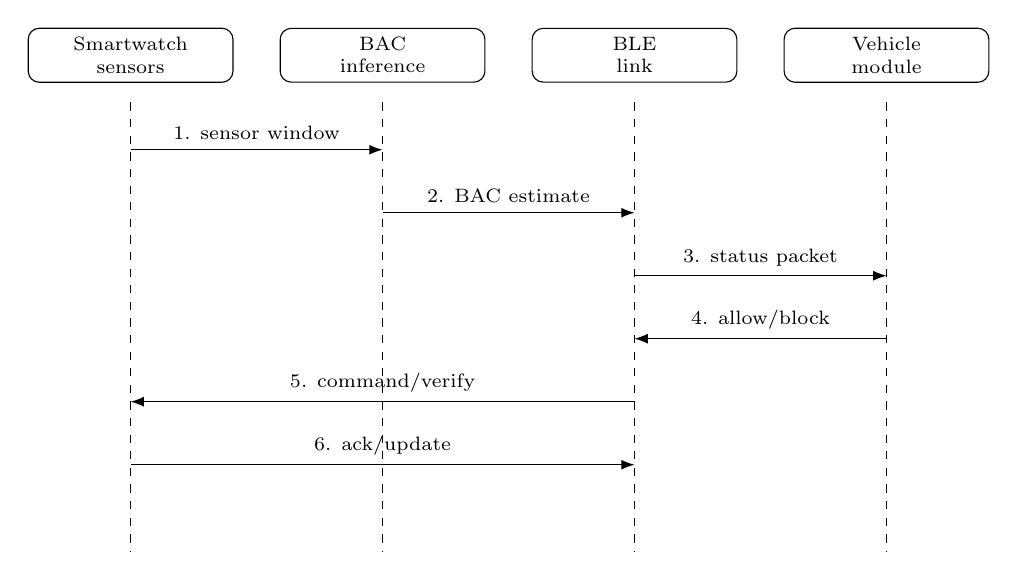
\begin{tikzpicture}[x=1cm,y=1cm,font=\scriptsize,>=Latex]
\node[draw, rounded corners, align=center, minimum width=2.6cm] (sw) at (1.3,0) {Smartwatch\\sensors};
\node[draw, rounded corners, align=center, minimum width=2.6cm] (ml) at (4.5,0) {BAC\\inference};
\node[draw, rounded corners, align=center, minimum width=2.6cm] (ble) at (7.7,0) {BLE\\link};
\node[draw, rounded corners, align=center, minimum width=2.6cm] (veh) at (10.9,0) {Vehicle\\module};

\draw[dashed] (1.3,-0.6) -- (1.3,-6.3);
\draw[dashed] (4.5,-0.6) -- (4.5,-6.3);
\draw[dashed] (7.7,-0.6) -- (7.7,-6.3);
\draw[dashed] (10.9,-0.6) -- (10.9,-6.3);

\draw[->] (1.3,-1.2) -- (4.5,-1.2) node[midway, above]{1. sensor window};
\draw[->] (4.5,-2.0) -- (7.7,-2.0) node[midway, above]{2. BAC estimate};
\draw[->] (7.7,-2.8) -- (10.9,-2.8) node[midway, above]{3. status packet};
\draw[->] (10.9,-3.6) -- (7.7,-3.6) node[midway, above]{4. allow/block};
\draw[->] (7.7,-4.4) -- (1.3,-4.4) node[midway, above]{5. command/verify};
\draw[->] (1.3,-5.2) -- (7.7,-5.2) node[midway, above]{6. ack/update};
\end{tikzpicture}

\caption{Operational sequence of sensing, BAC estimation, BLE transport
and ignition control.}
\label{fig:sequence}
\end{figure}

\section{Methods}
\subsection{Signal features}
Each inference window consists of 10 timesteps sampled at 30 s
intervals, resulting in a 5 min context window. Features are heart rate,
PPG signal quality, estimated EDA, skin temperature, ambient
temperature and humidity. Feature normalization uses
\begin{equation}
\label{eq:norm}
 x_{\mathrm{norm}} = \frac{x-\mu}{\sigma}.
\end{equation}

Because EDA sensors are not standard on Wear OS devices, EDA is
estimated from short-term heart rate variability
\begin{equation}
\label{eq:eda}
\mathrm{EDA}_{\mathrm{est}} = 3.0 + \frac{\sigma_{HR}}{5.0}.
\end{equation}

\subsection{Model architecture and loss}
The model uses a BiLSTM layer with attention over the 10-step sequence,
followed by two dense layers and a linear output. The safety-aware loss
adds a 5$\times$ penalty for false negatives relative to the legal
threshold $\tau = 0.08$ g/dL
\begin{equation}
\label{eq:loss}
\mathcal{L} = \mathrm{MSE}(y,\hat{y}) + 5\sum_i \mathbb{1}_{y_i>\tau\land\hat{y}_i<\tau}
(y_i-\hat{y}_i)^2.
\end{equation}

\subsection{Climate-adaptive calibration}
Ambient conditions affect skin conductivity and perspiration. A linear
adjustment corrects estimates using region-specific coefficients
\begin{equation}
\label{eq:cal}
\mathrm{BAC}_{\mathrm{cal}}=\mathrm{BAC}_{\mathrm{raw}} + \alpha_T(T_{\mathrm{amb}}-T_{\mathrm{base}})
+ \alpha_H\frac{H-50}{100}.
\end{equation}

\section{Implementation}
\subsection{Wear OS application}
The smartwatch application is written in Kotlin with an MVVM structure.
A circular buffer stores the latest 10 samples, and the TensorFlow Lite
interpreter outputs a BAC estimate and confidence score. Alerts are
classified into safe, warning and danger bands to guide user feedback.

\subsection{BLE protocol}
A custom GATT service transports the 20-byte BAC status packet shown in
Table~\ref{tab:bac_packet}. The packet includes timestamp, BAC estimate,
alert level, confidence and a flags byte for wear status and sensor
quality. Updates are transmitted every 30 s; the vehicle controller
blocks ignition if no valid update is received within 60 s.

\begin{table}[t]
\caption{BAC status packet format (20 bytes).}
\label{tab:bac_packet}
\centering
\small
\begin{tabular}{@{}llll@{}}
\toprule
Bytes & Field & Type & Description \\
\midrule
0--7 & Timestamp & uint64 & Unix epoch (ms) \\
8--11 & BAC & float32 & g/dL \\
12 & Alert level & uint8 & 0--3 \\
13 & Confidence & uint8 & 0--100\% \\
14 & Flags & uint8 & Wear, quality, battery \\
15--19 & MAC & byte[5] & Authentication tag \\
\bottomrule
\end{tabular}
\end{table}

The protocol specification supports AES-256-GCM for characteristic
payloads, while the current prototype relies on BLE pairing and reserves
space for a message authentication code. Full cryptographic enforcement
is required before deployment.

\subsection{Vehicle-side control}
The Arduino firmware implements a five-state machine: waiting for data,
ignition allowed, ignition blocked, connection lost, and override
active. Ignition is only enabled when BAC is below threshold, the watch
is worn, and sensor quality is acceptable. Any timeout, removal or
packet invalidation forces a blocked state.

\begin{table}[t]
\caption{Ignition control state machine.}
\label{tab:states}
\centering
\small
\begin{tabular}{@{}llllp{4cm}@{}}
\toprule
State & Relay & LED & Audio & Transition conditions \\
\midrule
WAITING\_FOR\_DATA & LOW & Blue blink & Silent & First valid packet \\
IGNITION\_ALLOWED & HIGH & Green solid & Silent & BAC $<$ 0.08 and watch worn \\
IGNITION\_BLOCKED & LOW & Red solid & 3 beeps & BAC $\geq$ 0.08 or watch removed \\
CONNECTION\_LOST & LOW & Blue blink & Silent & Timeout $>$ 60 s \\
OVERRIDE\_ACTIVE & HIGH & Green solid & 1 long beep & Manual override for 5 min \\
\bottomrule
\end{tabular}
\end{table}

\section{Experimental Setup}
Training uses 10,500 synthetic sequences with a 70/15/15 train/validation/test
split and early stopping. The synthetic data is generated from
literature-based correlations between alcohol consumption and
physiological changes. Evaluation metrics include MAE, RMSE, precision,
recall and false negative rate. Latency is measured end-to-end from
sensor acquisition to relay actuation on hardware. No human-subject data
are used in the current results.

\section{Results}
Table~\ref{tab:ml_results} summarizes model performance on the synthetic
holdout set. Table~\ref{tab:latency} reports end-to-end latency.

\begin{table}[t]
\caption{Model performance on synthetic test data.}
\label{tab:ml_results}
\centering
\small
\begin{tabular}{@{}llll@{}}
\toprule
Metric & Target & Achieved & Unit \\
\midrule
MAE & $\leq 0.010$ & 0.0082 & g/dL \\
RMSE & $\leq 0.015$ & 0.0124 & g/dL \\
Accuracy & $> 95$ & 97.3 & \% \\
Precision & $> 90$ & 94.1 & \% \\
Recall & $> 90$ & 96.8 & \% \\
False negative rate & $< 1$ & 0.7 & \% \\
\bottomrule
\end{tabular}
\end{table}

\begin{table}[t]
\caption{End-to-end latency breakdown.}
\label{tab:latency}
\centering
\small
\begin{tabular}{@{}lll@{}}
\toprule
Component & Operation & Latency (ms) \\
\midrule
Smartwatch & Sensing + preprocessing & 300 \\
Smartwatch & TFLite inference + calibration & 50 \\
BLE & Transmission & 150 \\
Arduino & Parsing + state update & 80 \\
\midrule
Total & End-to-end & 580 \\
\bottomrule
\end{tabular}
\end{table}

Resource use on the wearable device averages 18\% CPU utilization and a
2.8 MB memory footprint with 36 h of continuous monitoring on a typical
300 mAh battery.

\section{Discussion}
The low false negative rate reflects the asymmetric loss design and is
appropriate for a safety-critical application. These results should be
interpreted as feasibility evidence because training and testing are
performed on synthetic data. The results indicate that inference is not
the latency bottleneck; BLE transmission and signal processing dominate.
Climate calibration reduces error at extreme ambient conditions, but the
coefficients are population-level and do not account for individual
physiology.

\subsection{Clinical validation roadmap}
Future work will follow an IRB-approved protocol with controlled alcohol
administration and paired reference measurements. The validation plan
will report MAE, RMSE, threshold sensitivity at 0.08 g/dL, and
calibration error with 95\% confidence intervals computed by bootstrap
resampling. Baseline comparisons will include linear regression,
random-forest regression, an LSTM without attention, and the proposed
model without climate calibration. Cross-subject splits will be used to
test generalization, and Bland--Altman plots will quantify agreement
with reference BAC.

Security is currently limited by reliance on BLE pairing. Full
AES-256-GCM payload protection and replay defense should be integrated
before field trials. The largest scientific limitation is the use of
synthetic data; clinical validation with controlled alcohol
administration, IRB approval and demographic diversity is required to
establish generalizability and regulatory acceptance.

\section{Conclusion}
This paper provides a software blueprint for wearable BAC estimation and
ignition prevention, combining on-device ML inference, climate-adaptive
calibration, and a fail-safe vehicle control state machine. Prototype
results demonstrate low latency, compact model size and conservative
error behavior. The next steps are real-world data collection, security
hardening and formal safety validation to meet medical and automotive
regulatory requirements.

\section*{Acknowledgments}
The authors acknowledge the support of Amity University in Tashkent and
the supervision of Dr. Sudhanshu Tripathi.

\begin{thebibliography}{0}
\bibitem{uspat5736965} U.S. Patent No. 5,736,965, Alcohol Ignition
Interlock Device, filed March 15, 1996.

\bibitem{uspat7113834} U.S. Patent No. 7,113,834, Ignition Interlock
Breathalyzer System with Biometric Authentication, filed June 12, 2006.

\bibitem{inpat286703} Indian Patent No. 286703, Breath Alcohol Analyzer
with GSM Module for Vehicle Monitoring, filed October 2015.

\bibitem{fairbairn2021} C. E. Fairbairn and D. Kang, Transdermal alcohol
monitors: Research, applications, and future directions, in
{\it Handbook of Assessment in Clinical Gerontology}, 2nd ed.
(Academic Press, 2021), pp. 551--562,
\url{https://doi.org/10.1016/B978-0-12-816720-5.00014-1}.

\bibitem{verges2024} P. Verg{\'e}s {\it et al.}, Smartwatch-based prediction
of transdermal alcohol levels using hyperdimensional computing, in
{\it Proc. 10th IEEE World Forum on Internet of Things}, Ottawa, Canada
(2024), pp. 1--6, \url{https://doi.org/10.1109/WF-IoT62078.2024.10811151}.

\bibitem{lombardo2020} L. Lombardo, S. Grassini, M. Parvis, N. Donato
and A. Gullino, Ethanol breath measuring system, in {\it Proc. IEEE
International Symposium on Medical Measurements and Applications}
(2020), pp. 1--6, \url{https://doi.org/10.1109/MEMEA49120.2020.9137215}.

\bibitem{das2023} D. K. Das, A. P. Reddy, S. K. Ajay, D. Dhanalakshmi,
S. Hariharan and V. Kukreja, Vehicle ignition locking system and
analysis for accident prevention by blood alcohol content measurement,
in {\it Proc. International Conference on Smart Systems and Advanced
Computing} (2023), pp. 1494--1499,
\url{https://doi.org/10.1109/ICSSAS57918.2023.10331684}.

\bibitem{sensors2024} Wearable alcohol monitoring system with vehicular
interface, {\it Sensors} {\bf 24} (2024), Article 4233,
\url{https://www.mdpi.com/1424-8220/24/13/4233}.

\bibitem{sensors2023} Vehicle and driver monitoring system using
on-board and remote sensors, {\it Sensors} {\bf 23} (2023), Article 814,
\url{https://www.mdpi.com/1424-8220/23/2/814}.

\bibitem{alcowatch2025} Smartwatch-based ecological momentary assessment
for high-temporal-density, longitudinal measurement of alcohol use
(AlcoWatch): Feasibility evaluation, {\it JMIR Formative Research}
{\bf 9} (2025), Article e63184,
\url{https://formative.jmir.org/2025/1/e63184/}.
\end{thebibliography}

\end{document}
